\documentclass[final,t]{beamer}
\mode<presentation>
{
%  \usetheme{Warsaw}
%  \usetheme{Aachen}
%  \usetheme{Oldi6}
%  \usetheme{I6td}
  \usetheme{I6dv}
%  \usetheme{I6pd}
%  \usetheme{I6pd2}
}
% additional settings
\setbeamerfont{itemize}{size=\normalsize}
\setbeamerfont{itemize/enumerate body}{size=\normalsize}
\setbeamerfont{itemize/enumerate subbody}{size=\normalsize}
% additional packages
\usepackage{ragged2e}
\usepackage[ampersand]{easylist}
\usepackage{lipsum}
\usepackage{times}
\usepackage{amsmath,amsthm, amssymb, latexsym}
\usepackage{exscale}
%\boldmath
\usepackage{booktabs, array}
%\usepackage{rotating} %sideways environment
\usepackage[english]{babel}
\usepackage[latin1]{inputenc}
\usepackage[orientation=landscape,size=custom,width=109.728,height=91.44,scale=1]{beamerposter}
\addtobeamertemplate{block begin}{}{\justifying}
\listfiles
\graphicspath{{figures/}}
% Display a grid to help align images
%\beamertemplategridbackground[1cm]

\title{\huge scikit-bio: a Python library for bioinformaticians and data scientists}
\author{Evan T. Bolyen, The scikit-bio Development Team and J. Gregory Caporaso}
\institute{Affiliations go here}

% abbreviations
\usepackage{xspace}
\makeatletter
\DeclareRobustCommand\onedot{\futurelet\@let@token\@onedot}
\def\@onedot{\ifx\@let@token.\else.\null\fi\xspace}
\def\eg{{e.g}\onedot} \def\Eg{{E.g}\onedot}
\def\ie{{i.e}\onedot} \def\Ie{{I.e}\onedot}
\def\cf{{c.f}\onedot} \def\Cf{{C.f}\onedot}
\def\etc{{etc}\onedot}
\def\vs{{vs}\onedot}
\def\wrt{w.r.t\onedot}
\def\dof{d.o.f\onedot}
\def\etal{{et al}\onedot}
\makeatother

%%%%%%%%%%%%%%%%%%%%%%%%%%%%%%%%%%%%%%%%%%%%%%%%%%%%%%%%%%%%%%%%%%%%%%%%%%%%%%%%%%%%%%%%%%%%%%%%%%%%%%%%%%%%
%%%%%%%%%%%%%%%%%%%%%%%%%%%%%%%%%%%%%%%%%%%%%%%%%%%%%%%%%%%%%%%%%%%%%%%%%%%%%%%%%%%%%%%%%%%%%%%%%%%%%%%%%%%%
\begin{document}
\begin{frame}{}
  \begin{columns}[t]
    \begin{column}{.3\linewidth}
        \begin{alertblock}{
\includegraphics[width=1\linewidth]{assets/skbio}\newline\newline}
          scikit-bio is an open-source, BSD-licensed python package providing data structures, algorithms and educational resources for bioinformatics.
          \newline\newline
        \end{alertblock}

        \begin{block}{GOALS}
            \large{\begin{itemize}
                \item[$\bullet$] Make building tools like QIIME easier.
                \item[$\bullet$] Provide Data Structures and Algorithms.
                \item[$\bullet$] Domain specific API that maps biological vocabulary to implementation.
                \item[$\bullet$] Extensive supporting documentation.
                \item[$\bullet$] Optimized wherever possible.
                \item[$\bullet$] Rigorously tested.
            \end{itemize}}
        \end{block}

        \begin{block}{\uppercase{Current Users of scikit-bio}}

            \large{\begin{itemize}
              \item[$\bullet$] QIIME 1.9 \hfill \\
              - Quatitative Insights Intro Microbial Ecology
              \item[$\bullet$] ghosttree
          \end{itemize}}
        \end{block}

        \begin{block}{\uppercase{Future Users of scikit-bio}}
            \large{\begin{itemize}
              \item[$\bullet$] QIIME 2
              \item[$\bullet$] qiita
          \end{itemize}}
        \end{block}





      %%%%%%%%%%%%%%%%%%%%%%%%%%%%%%%%%%%%%%%%%%%%%%%%%%%%%%%%%%%%%%%%%%%%%%%%%%%%%%%%%%%%%%%%%%%%%%%%%%%%%%%%%%%%


    \end{column}
    \begin{column}{.3\linewidth}
        %%%%%%%%%%%%%%%%%%%%%%%%%%%%%%%%%%%%%%%%%%%%%%%%%%%%%%%%%%%%%%%%%%%%%%%%%%%%%%%%%%%%%%%%%%%%%%%%%%%%%%%%%%%%


        \begin{block}{\uppercase{Documentation}}
            Documentation for scikit-bio is available in many forms:
            \newline\newline
            \begin{columns}
                \begin{column}{.45\linewidth}
                    \begin{minipage}[c][15cm][c]{\linewidth}
                        \href{http://scikit-bio.org}{\color{blue}\underline{scikit-bio.org}}
                        \newline\newline
                        Our website provides the API documentation is an easy to read form.

                    \end{minipage}
                    \begin{minipage}[c][15cm][c]{\linewidth}
                        \href{http://applied-bioinformatics.org}{\color{blue}\underline{applied-bioinformatics.org}}
                        \newline\newline
                        Introduction to Applied Bioinformatics
                    \end{minipage}
                    \begin{minipage}[c][15cm][c]{\linewidth}
                        \href{http://scikit-bio.org/cookbook}{\color{blue}\underline{scikit-bio.org/cookbook}}
                        \newline\newline
                    \end{minipage}
                \end{column}
                \begin{column}{.45\linewidth}
                    \begin{minipage}[c][15cm][c]{\linewidth}
                    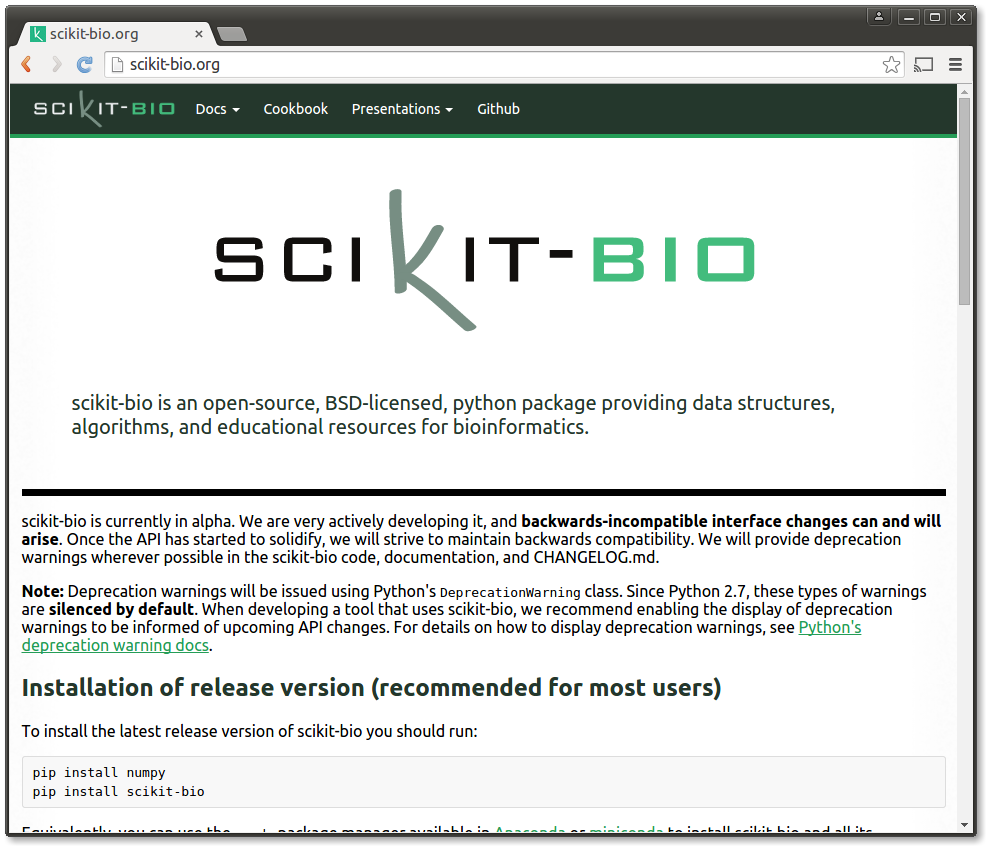
\includegraphics[width=1\linewidth]{assets/website}\\
                \end{minipage}
                        \begin{minipage}[c][15cm][c]{\linewidth}
                    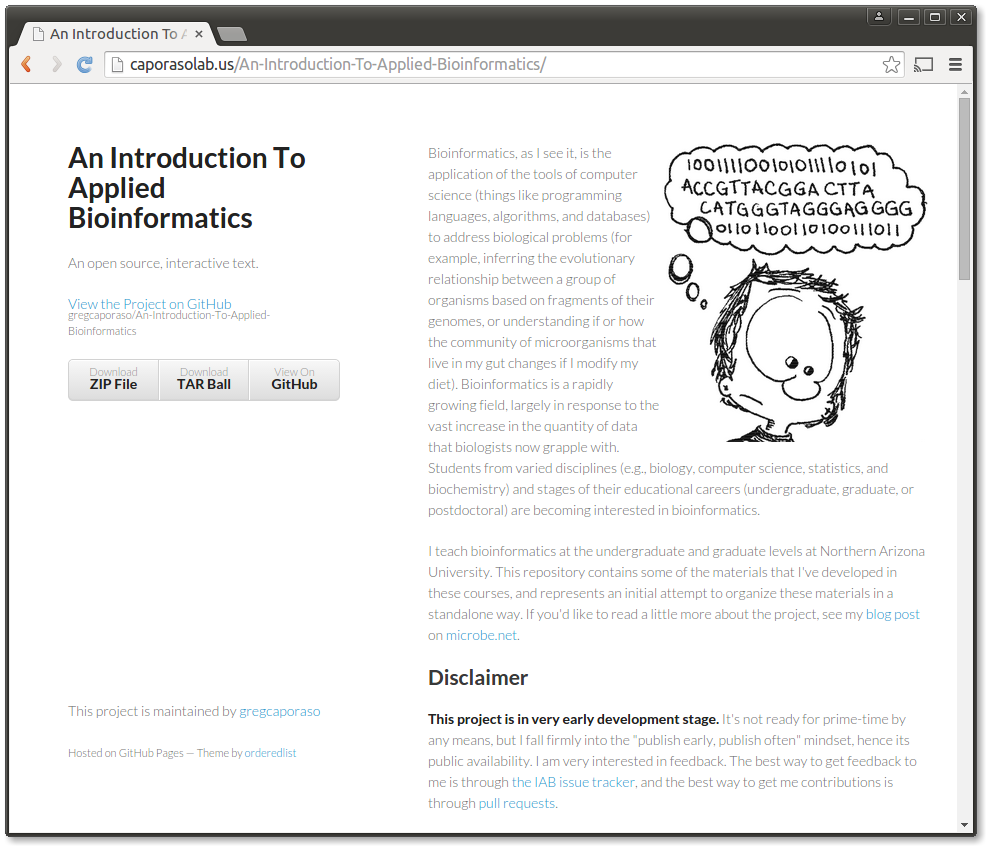
\includegraphics[width=1\linewidth]{assets/iab}\\
                \end{minipage}
                        \begin{minipage}[c][15cm][c]{\linewidth}
                    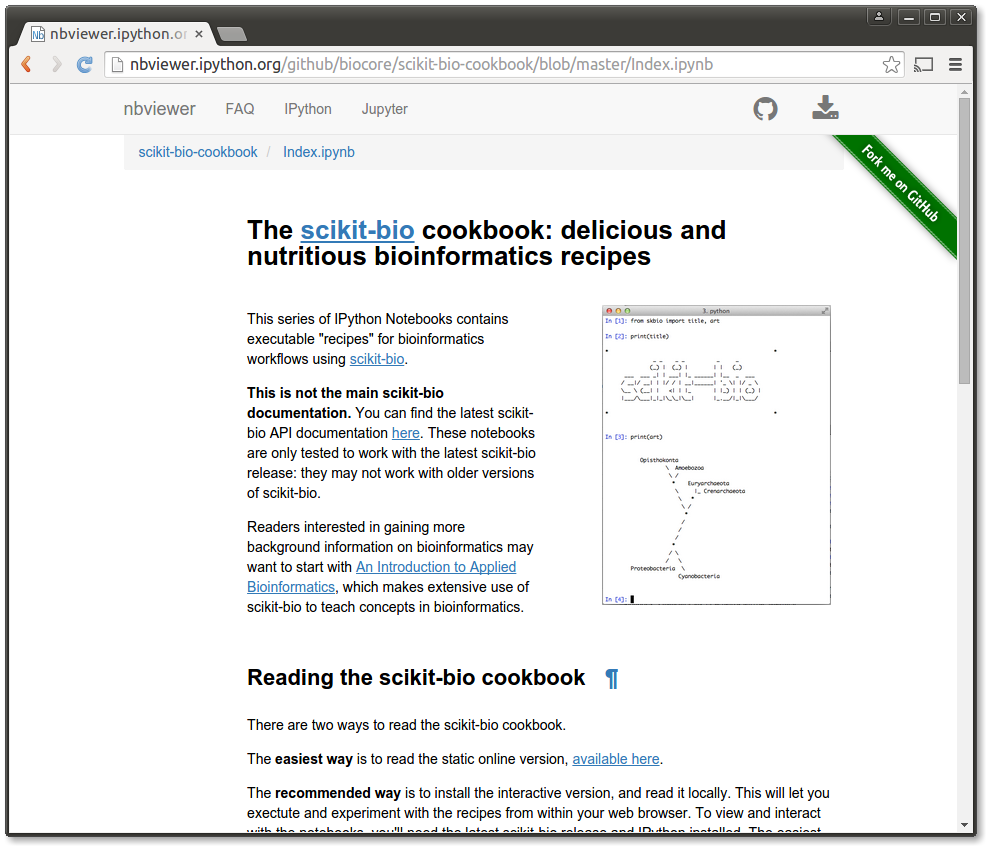
\includegraphics[width=1\linewidth]{assets/cookbook}
                \end{minipage}
                \end{column}
            \end{columns}

        \end{block}

    \end{column}

    %%%%%%%%%%%%%%%%%%%%%%%%%%%%%%%

    \begin{column}{.3\linewidth}

        %%%%%%%%%%%%%%%%%%%%%%%%%%%%%%%%%%%%%%%%%%%%%%%%%%%%%%%%%%%%%%%%%%%%%%%%%%%%%%%%%%%%%%%%%%%%%%%%%%%%%%%%%%%%

          \begin{block}{\uppercase{Convert Fasta/Qual to FastQ}}
            There are a lot of file formats in bioinformatics, one common challenge is taking data encoded in one format, and transforming it into something else (often a different format).
            \newline\newline
            \python{assets/py/convert_fastq.py}
            \newline
            This streamed full records one at a time into a new format.\newline\newline
            Another exciting feature of scikit-bio are ``sniffers'' which can automatically detect the format of a file and read it into a data-structure.

          \end{block}

          %%%%%%%%%%%%%%%%%%%%%%%%%%%%%%%%%%%%%%%%%%%%%%%%%%%%%%%%%%%%%%%%%%%%%%%%%%%%%%%%%%%%%%%%%%%%%%%%%%%%%%%%%%%%

          \begin{block}{\uppercase{Find Pairwise Similarity}}
            Short explanation on why this is useful.
            \newline\newline
            \python{assets/py/pairwise_similarity.py}
            \newline\newline
            \ttfamily{0.591048436542}
          \end{block}

        \begin{columns}
        \begin{column}{.02\linewidth} \end{column}
            \begin{column}{.48\linewidth}
                \begin{block}{\uppercase{References}}
                    References will go here
                \end{block}
            \end{column}
            \begin{column}{.48\linewidth}
                \begin{block}{\uppercase{Acknowledgements}}
                    Acknowledgements will go here.
                \end{block}
            \end{column}
        \end{columns}
%%%%%%%%%%%%%%%%%%%%%%%%%%%%%%%%%%%%%%%%%%%%%%%%%%%%%%%

    \end{column}
  \end{columns}
  \begin{columns}
      \begin{column}{.02\linewidth} \end{column}
      \begin{column}{.9625\linewidth}
          \begin{block}{TAKEAWAY}
              Test
          \end{block}
      \end{column}
      \begin{column}{.0175\linewidth} \end{column}
  \end{columns}
\end{frame}

\end{document}


%%%%%%%%%%%%%%%%%%%%%%%%%%%%%%%%%%%%%%%%%%%%%%%%%%%%%%%%%%%%%%%%%%%%%%%%%%%%%%%%%%%%%%%%%%%%%%%%%%%%
%%% Local Variables:
%%% mode: latex
%%% TeX-PDF-mode: t
%%% End:
